%!TEX root = /Users/markelikalderon/Documents/Git/formwithoutmatter/formwithoutmatter.tex
\chapter{The Generation of the Hues} % (fold)
\label{cha:the_generation_of_the_hues}

\section{Light and Dark} % (fold)
\label{sec:introduction}
The presence of the fiery substance illuminates the potentially transparent me\-di\-um. White (\emph{leukon}) corresponds to the presence of this determinant of what is actually transparent. Conversely, black (\emph{melaton}) corresponds to its absence. The absence of the fiery substance darkens the potentially transparent medium. White and black are thus associated with a fundamental condition on the visibility of remote external particulars. No doubt in part because of this Aristotle attempts to explain the other hues in terms of the ratio of white and black. He considers three such accounts, in terms of (1) juxtaposition, (2) overlap, and (3) mixture, advocating the third. On all three accounts chromatic hues are determined by white and black in various ratios, the accounts differing only in how these ratios are implemented. 

The fundamental idea common to all three accounts can seem surprising. How can the ratio of white and black result in something appearing red? Would it not instead appear gray? Thus \citet[210]{Hett:1936fk} writes that Aristotle's ``doctrine could hardly have survived a few experiments with pigments''. If Aristotle's account were disconfirmable by elementary experiments with pigment mixtures, then why did he not investigate the matter? Was it merely to avoid Plato's charge of impiety?
\begin{quote}
    There will be no difficulty in seeing how and by what mixtures the colors derived from these are made according to the rules of probability. He, however, who should attempt to verify all this by experiment would forget the difference between human and divine nature. For God only has the knowledge and also the power which are able to combine many things into one and again resolve the one into many. But no man either is or ever will be able to accomplish either the one or the other operation. (Plato, \emph{Timaeus} 68d)
\end{quote}
Aristotle's account of the generation of the hues may be surprising, but it would be wrong to prematurely dismiss it. 

The first thing to observe is that \emph{leukon} and \emph{melaton} are better understood as light and dark, rather than white and black. There is a general tendency in Greek color vocabulary to classify colors in terms of relative brightness rather than hue \citep[see][]{Gladstone:1858fk,Platnauer:1921bh,Osbourne:1968vn,Lloyd:2007fk}. Traces of such a usage exist in English. Thus we speak of white wine and white people, though neither are white in hue. Similarly neither black people nor black grapes are black in hue. This usage in English, however, does not seem to be perfectly general but is rather lexically determined. It is not the case that for any noun \( N \), the occurrence of ``white'' in \( \ulcorner [white_{Adj}][N_{N}] \urcorner \) can be interpreted in terms of relative brightness instead of hue. The availability of such an interpretation seems to be limited to the adjective's application to certain nouns. The more general usage in Greek is philosophically significant, for it transforms Aristotle's claim. Aristotle is not claiming that the hues are determined by the ratio of white and black, but that they are determined by the ratio of light and dark. Experiments with pigment mixtures are irrelevant to the truth of this latter claim. Thus, Aristotle need not have risked Plato's charge of impiety as Hett recomends. Not only is the thought that the hues are determined by the ratio of light and dark not disconfirmable by impious experimentation, it is independently plausible. Indeed, as I will argue below, it is an ancient prefiguration of modern reflectance theories \citep[see][]{Hilbert:1987jq}.

Two further considerations are relevant. First, there are a range of observable phenomena that support Aristotle's fundamental claim that a ratio of white and black or light and dark can give rise to chromatic appearances. Importantly, Aristotle himself provides an example. Second, Aristotle's account has ancient precedent. Thus when Theophrastus discusses Democritus's view that there are four primary colors (understood as simple colors in terms of which all other colors are to be explained), he contrasts it with the then dominant view that white and black are the two primary colors:
\begin{quote}
    But first of all, his increase of the number of primaries presents a difficulty; for the other investigators propose white and black as the only simple colours. (\emph{De Sensibus} 79; DK 68\textsc{a}135; \citealt{Stratton:1917vn})
\end{quote}
It is reasonable to suppose that Aristotle's account of the generation of the hues draws on this pre-Democritean tradition. Before discussing Aristotle's account of the generation of the hues, then, I will review some empirical support for its central idea, and will discuss the precedent for this doctrine in Parmenides and Empedocles.

% section introduction (end)

\section{Empirical Support} % (fold)
\label{sec:empirical_support}
In 1894, an English toy maker, Charles Benham, devised a top adorned with a black and white pattern (see Figure~\ref{fig:2}). Sold through Messrs. Newton and Co., an announcement of the ``Artificial Spectrum Top'' was published in \emph{Nature}:
	\begin{quote}
		The top consists of a disc, one half of which is black, while the other half has twelve arcs of concentric circles drawn upon it. Each arc subtends an angle of forty-five degrees. In the first quadrant there are three such concentric arcs, in the next three more, and so on; the only difference being that the arcs are parts of circles of which the radii increase in arithmetical progression. Each quadrant thus contains a group of arcs differing in length from those of the other quadrants. The curious point is that when this disc is revolved, the impression of concentric circles of different colors is produced upon the retina. If the direction of rotation is reversed, the order of these tints is also reversed. \citep{Benham:1894kx}
	\end{quote}
Specifically, if rotated clockwise, the innermost arcs form reddish rings, the next greenish rings, the next light blue rings, and the outermost arcs form violet rings. If rotated counterclockwise, the pattern is reversed with the innermost arcs now forming violet rings and the outermost reddish rings. The apparent colors of Benham's spinning disk are the ``subjective colors'' first described by \citep{Fechner:1838vn} and, hence, are also sometimes described as ``Fechner-Benham colors''.

\begin{figure}[ht]
    \begin{center}
        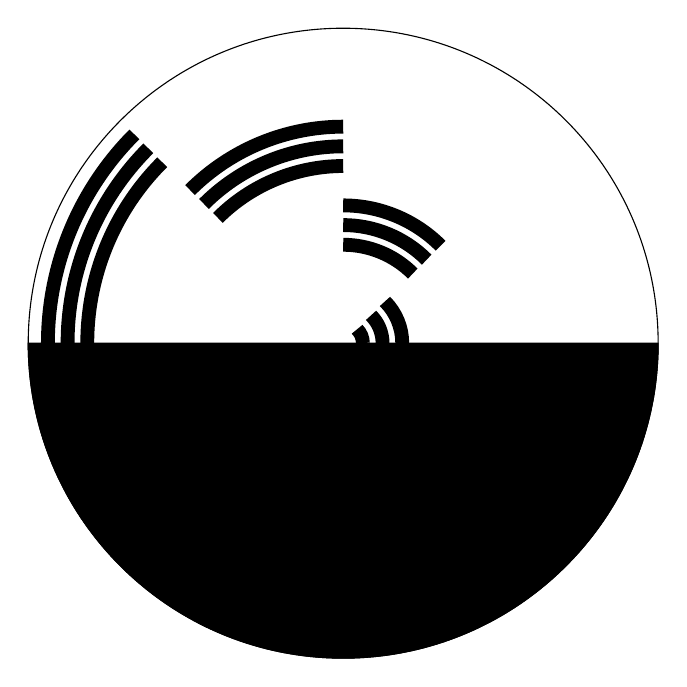
\begin{tikzpicture}
			\draw (0,0) circle (4cm);
			\filldraw[fill=black] (0,0) -- (4cm,0cm) arc (0:-180:4cm) --cycle;
			\draw[line width=5pt] (canvas polar cs:angle=0,radius=0.25cm) arc (0:45:0.25cm);
			\draw[line width=5pt] (canvas polar cs:angle=0,radius=0.50cm) arc (0:45:0.50cm);
			\draw[line width=5pt] (canvas polar cs:angle=0,radius=0.75cm) arc (0:45:0.75cm);
			\draw[line width=5pt] (canvas polar cs:angle=45,radius=1.25cm) arc (45:90:1.25cm);
			\draw[line width=5pt] (canvas polar cs:angle=45,radius=1.50cm) arc (45:90:1.50cm);
			\draw[line width=5pt] (canvas polar cs:angle=45,radius=1.75cm) arc (45:90:1.75cm);
            \draw[line width=5pt] (canvas polar cs:angle=90,radius=2.25cm) arc (90:135:2.25cm);
			\draw[line width=5pt] (canvas polar cs:angle=90,radius=2.50cm) arc (90:135:2.50cm);
			\draw[line width=5pt] (canvas polar cs:angle=90,radius=2.75cm) arc (90:135:2.75cm);
			\draw[line width=5pt] (canvas polar cs:angle=135,radius=3.25cm) arc (135:180:3.25cm);
			\draw[line width=5pt] (canvas polar cs:angle=135,radius=3.50cm) arc (135:180:3.50cm);
			\draw[line width=5pt] (canvas polar cs:angle=135,radius=3.75cm) arc (135:180:3.75cm);
		\end{tikzpicture}
    \end{center}
    \caption{The Benham Disk or ``Artificial Spectrum Top''}
    \label{fig:2}
\end{figure}

Consider a puzzling aspect of the subjective colors of the Benham disk. Each of the spinning arcs reflect light with the same spectral content and with equal average luminance. In advance of observing the spinning disk, one might reasonably expect the spinning arcs to appear as gray rings of equal brightness. Why, then, do the rings appear reddish, greenish, light blue, and violet? The subjective colors of the Benham disk are not completely understood \citep[for a review of some of the color science see][]{Campenhausen:1995yq}. However, this much is clear: The innermost ring appearing reddish is the result of the visual system integrating temporal inhomogeneities presented by the spinning disk. Presentations of black and white stimuli altering at a particular temporal ratio elicits a chromatic response in normal human perceivers. 

This basic principle was used in a prototype color television broadcasting system \citep[]{Butterfield:1968uq,Butterfield:1970kx}. Developed by James F. Butterfield (who studied philosophy at the University of Chicago as an undergraduate), the broadcasting system consists of the Butterfield color encoder that produces a monochromatic signal that when broadcast and displayed on a black-and-white monitor presents a chromatic appearance. The Butterfield encoder extracts a monochromatic signal from the colored scene by passing the light from the scene through cyan, magenta, and yellow filters. The filters themselves are arranged in, what is in effect, a modified Benham Disk (see Figure~\ref{fig:3}). The bottom half of the filter is opaque with the colored filters fanned across the top half. The filters thus form a disk which is rotated. A colored object will appear black when seen through a filter of a complementary color. This and the opaque half of the rotating disk produces a pulsed black-and-white signal that elicits a chromatic response in normal human perceivers. The system produced good skin tones but unmixed hues, especially red, tended to flicker. The initial public demonstration was, by all accounts, startling:
\begin{quote}
    When electronic color was first publicly demonstrated in the Los Angeles area over KNXT, no prior announcement had been made at the request of a soft-drink manufacturer sponsoring the test. The beverage firm wanted its color commercials to be a complete surprise to viewers of black-and-white receivers. And, the telecasts were that, to say the very least. Within hours of the electronic-color broadcast, thousands of viewers began asking the same question, ``What happened? Did I really see color on my black-and-white receiver? Or am I having hallucinations?'' \citep[]{Griffin:1968fk}
\end{quote}
The power to demand such attention did not go unnoticed. The final public demonstration was an Eva Perón political advertisement.

\begin{figure}[htbp]
    \centering
        
\includegraphics[scale=.55]{graphics/color_encoder.jpg}
    \caption{Butterfield color encoder \citep{Shatavsky:1968vn}}
    \label{fig:3}
\end{figure}

That the pulsed black-and-white signal produced by the Butterfield color encoder gives rise to a chromatic appearance is once again the result of the visual system integrating temporal inhomogeneities. However, these temporal inhomogeneities are not the result of spatial movement of the object of perception, but rather due to the qualitative alterations over time of a stationary object. Each involves the presentation of white and black stimuli altering at a particular temporal ratio eliciting a chromatic response in normal human perceivers. They differ in how that temporal ratio is implemented---by the motion of an object whose parts qualitatively differ or by the qualitative alteration over time of a stationary object. 

Stated so abstractly it is easy to see that there is a third possibility. If the temporal ratio that determines a given chromatic appearance can be implemented by the motion of a black and white object, the perceivers motion relative to a black and white object should do so as well. And indeed it can. Our eyes constantly scan the scene with involuntary saccades. Scanning a stationary black and white object can give rise to chromatic appearance \citep[72]{Hardin:1993kn}. Thus Sorabji claims that certain Bridget Riley paintings are an example:
\begin{quote}
    The English painter, Bridget Riley, has produced pictures in which black and white are juxtaposed, in long ribbons \ldots\ When people look at these black and white ribbons, many are able to see all sorts of colours appearing. \citep[295]{Sorabji:2022qf}
\end{quote}
These chromatic appearances are the result of the visual system integrating temporal inhomogeneities that result from the eye involuntarily moving across a stationary black and white object.

These examples involve artifacts and technology unavailable at Aristotle's time. And while they may make plausible for \emph{us} that ratios of white and black or light and dark can, sometimes at least, give rise to chromatic appearances, they could not have done so for Aristotle. What empirical observation available to Aristotle could have made vivid for him the possibility that chromatic appearances are the result of the ratio of light and dark in the perceived scene? An example discussed in the last chapter could give rise to the relevant experience. The sun is white, but it appears red when seen through fog or a cloud of smoke (\emph{De Sensu} 3 440\( ^{a} \)10--11).  The white sun, when superimposed by black particles suspended in the intervening transparent medium, looks red. The reduction of the sun's brilliance by the intervening particulate matter of the smoke results in the sun's crimson appearance. What is presently important is a general feature of Aristotle's example: that a reduction of the sun's brilliance results in a chromatic appearance. That provides direct partial support for the claim that a proportion of light and dark can give rise to a chromatic appearance. % In this regard, the point of Aristotle's example in its context, that the red appearing proportion of light and dark is the result of overlap or sumperimposition, is of less importance.  

% section empirical_support (end)

\section{Parmenides} % (fold)
\label{sec:parmenides}
Theophrastus (\emph{De Sensibus} 79; DK 68\textsc{a}135) alludes to a pre-Democritean tradition according to which white and black are the primary colors, the colors in terms of which all other colors are to be explained. While Theophrastus does not name any particular thinker belonging to this tradition, one may reasonably speculate. In his notorious study, among the five ``signs of the immaturity'' of the Homeric color scheme, Gladstone cites the following:  
\begin{quote}
    The vast predominance of the most crude and elemental forms of colour, black and white, over every other, and the decided tendency to treat other colours as simply intermediate modes between these two extremes. \citep[458]{Gladstone:1858fk}
\end{quote}
One can reasonably accept Gladstone's observation about the structure of the Ho\-meric color scheme, while bracketing any conclusions about relative deficiencies in the Greek's capacity to discriminate color. (Amusingly, \citealt[162]{Platnauer:1921bh}, while tempted by Gladstone's attribution of perceptual deficit to the ancient Greeks, accuses them instead of having bad taste in color composition.) If we do, then arguably the pre-De\-mo\-cri\-tean tradition that Theophrastus alludes to has Homeric roots. Let us selectively examine this ancient tradition by attending to two key figures familiar to Aristotle, Parmenides and Empedocles (though the inclusion of the latter is controversial).

In the prologue to his poem, the goddess promises to reveal to Parmenides two things, the Way of Truth and the Way of Mortal Opinion. The doctrines of the latter she assures him are false; nevertheless, Parmenides must learn these too (DK 28\textsc{b}1 31). The Way of Mortal Opinion is an account of the world ``as it appears'' (DK 28\textsc{b}8 60; \citealt[155]{McKirahan:1994ve}), and the goddess presents it to Parmenides ``so that no mortal opinion may ever overtake'' him (DK 28\textsc{b}8 61; \citealt[155]{McKirahan:1994ve}). The Way of Mortal Opinion is a cosmology in the Milesian tradition, though Parmenides is not expounding the views of any particular Milesian cosmologist \citep[on Parmenides and Milesian cosmology see][]{Kahn:1994qf}. Rather, he is presenting what is, by his lights, the best account that can be given along those lines. Traditional Milesian cosmologies tend to be monistic, but the Way of Mortal Opinion posits two fundamental and irreducible principles that stand in opposition, Fire and Night or light and dark (DK 28\textsc{b}8 53--61, 28\textsc{b}9). The thought seems to be this. Having shown, in the Way of Truth, that monism is inconsistent with appearances, the Way of Mortal Opinion must posit a plurality of principles in opposition, if it is to accommodate the plurality and opposition encountered in the world as it appears in sensory experience:
\begin{verse}
    For they made up their minds to name two forms,\\ 
    Of which it is not right to name one---in this they have gone astray---\\
    And they distinguished things opposite in body, and established signs\\
    Apart from one another---for one, the aetherial fire of flame,\\
    Mild, very light, the same as itself in every direction,\\
    But not the same as the other; but that other one, in itself\\
    Is opposite---dark night, a dense and heavy body.\\
    I declare to you all the ordering as it appears,\\
    So that no mortal opinion may ever overtake you.
\end{verse}
\begin{verse}
    But since all things have been named light and night\\
    And the things which accord with their powers have been assigned to these things and those,\\
    All is full of light and obscuring night together,\\
    of both equally, since neither has no share.\\
    (Parmenides, DK 28\textsc{b}8 53--9 4; \citealt[155]{McKirahan:1994ve})
\end{verse}
The two principles, Fire and Night, of the Way of Mortal Opinion, have attributes called ``signs''. Like Fire and Night themselves, the attributes of these principles stand in opposition. Fire is bright, Night is dark; Fire is lightweight, Night is heavy, and so on. Fire and Night may have further attributes not listed here; much of the Way of Mortal Opinion is missing. A sense of its ambition and importance, however, is provided by Plutarch:
\begin{quote}
    But Parmenides \ldots\ has actually made a cosmic order, and by blending as elements the light and the dark produces out of them and by their operation the whole world of sense. Thus he has much to say about earth, heaven, sun, moon, and stars, and has recounted the genesis of man; and for an ancient natural philosopher---who has put together a book of his own, and is not pulling apart the book of another---he has left nothing of real importance unsaid. (Plutarch, \emph{Adversus Colotem} 1114 b--c; \citealt[231]{Einarson:1967zr})
\end{quote}
The attributes of the fundamental principles of the Way of Mortal Opinion are sensible qualities arrayed in opposing pairs of contraries. In contrast, the attributes of the one being of the Way of Truth are not sensible (\emph{aistheton}) but intelligible (\emph{noeton}) properties (such as form or unity). 

Arguably, the cosmology of Fire and Night posited by the Way of Mortal Opinion is prefigured in the prologue of the poem. On his journey to meet the goddess, Parmenides, escorted by the daughters of the Sun, travels from Night to Day:
\begin{verse}
    \ldots\ the daughters of the Sun\\
    Were hastening to escort <me> after leaving the house of Night\\
    For the light, having pushed back the veils from their heads with their hands.\\ 
    (Parmenides, DK 28\textsc{b}1 8--10; \citealt[151]{McKirahan:1994ve})
\end{verse}
But before they can meet the goddess they must pass through the gates of the roads of Night and Day:
\begin{verse}
    There are the gates of the roads of Night and Day,\\
    And a lintel and a stone threshold contains them.\\ 
    High in the sky they are filled by huge doors\\
    Of which avenging Justice holds the keys that fit them.\\
    (Parmenides, DK 28\textsc{b}1 11--13; \citealt[151]{McKirahan:1994ve})
\end{verse}
Parmenides must leave the sensible world governed by alternations of Night and Day, to the intelligible world where a goddess awaits to reveal to him the Way of Truth.

If, according to the Way of Mortal Opinion, the entirety of sensible world---in which appear ``earth, heaven, sun, moon, and stars''---is ultimately explained in terms of light and dark in opposition, then the qualities of material objects that appear in sensory experience are themselves to be explained in these terms. Since colors are qualities of material objects that appear in sensory experience, they are themselves to be explained in terms of the ``blending'' of light and dark. Whether or not Theophrastus had Parmenides in mind, Parmenides straightforwardly belongs to the pre-Democritean tradition that postulates white and black or light and dark as the primary colors.

% section parmenides (end)

\section{Empedocles} % (fold)
\label{sec:empedocles}

It is at least arguable that Theophrastus did in fact have Empedocles in mind when alluding to this pre-Democritean tradition. Despite extensive discussion of Empedocles' views about sensory experience and its objects, Theophrastus does not make the parallel charge against Empedocles that he makes against Democritus (\emph{De Sensibus} 79; DK 68\textsc{a}135; \citealt{Stratton:1917vn}). Moreover, as we have seen, Theophrastus complains that while Empedocles has explained the perception of white and black he has failed to explain the perception of the other hues (\emph{De Sensibus} 17; \citealt{Stratton:1917vn}). This is strong defeasible evidence that Theophrastus took Empedocles to be among the thinkers who take white and black or light and dark as the primary colors (albeit with limited success, at least by Theophrastus' lights).

In contrast with Parmenidean monism, Empedocles postulates the existence of four ``roots'' or elements---water, earth, air, and fire---and two principles---\-Love and Strife. Whereas Love, the principle of harmony, has the power to unite, Strife, the principle of disorder, has the power to divide. According to Empedocles, things are colored because of the combination of elements that result from Love overcoming Strife to the extent that it does:
\begin{verse}
    And if, concerning these things, your conviction is in any way wanting,\\
    as to how from the blending of water and earth and aither and sun\\
    the forms and colours of mortals came to be,\\
    which have now come to be, fitted together by Aphrodite.
    (DK \textsc{b}71; \citealt[74 249]{Inwood:2001ve})
\end{verse}
The forms and colors of objects we encounter in sensory experience are to be explained in terms of the combination of the elements that result from Love's influence counteracting the operation of Strife.

\citet[222]{Wright:1981zr} suggests that the reference to form and color is a deliberate echo of an earlier fragment:
\begin{verse}
    As when painters adorn votive offerings,\\
    men well-learned in their craft because of cunning,\\
    and so when they take in their hands many-coloured pigments,\\
    mixing them in harmony, some more, others less,\\
    from them they prepare forms resembling all things,
    making trees and men and women\\
    and beasts and birds and water-nourished fish\\
    and long-lived gods, first in their prerogatives.\\
    In this way let not deception overcome your thought organ\\
    that the source of mortal things, as many as have become obvious---countless---is anything else,\\
    but know these things clearly, having heard the story from a god.\\ 
    (DK \textsc{b}23; \citealt[27 231]{Inwood:2001ve})
\end{verse}
However, the two fragments seem to be making different points. Empedocles in this earlier fragment describes the generation of the objects we encounter in the sensible world by analogy with painting. Just as painters can represent everything in the sensible world by combining pigments in various proportions, Love and Strife can generate everything in the sensible world by combining the elements in various proportions. However, unlike the later fragment (DK \textsc{b}71) no specific mention is made about the colors of the generated objects or how they are the result of the combination of elements. Whereas the earlier fragment (DK \textsc{b}23) claims that a combination of a few colors suffice to represent the forms and colors encountered in the sensible world, the latter fragment (DK \textsc{b}71) claims that a combination a few elements suffice for the forms and colors encountered in the sensible world.

The painting analogy remains instructive, however. Specifically, it sheds light on the sense in which the combination of a few colors suffice to represent all the colors that appear in sensory experience. This is important since in the context of Empedocles' analogy, this is the sense in which the elements combine. And given the latter fragment (DK \textsc{b}71), the elements when combined in this sense suffice for the form and color of all things. First, observe that, despite their manifest plurality, the ``roots'' or elements are otherwise Parmenidean beings---they do not admit of alteration, growth, or decay. Change as we experience it is the result of different combinations of these unchanging elements:
\begin{verse}
    I shall tell you something else. There is no growth of any or all mortal things\\
    nor any end in destructive death,\\
    but only mixture and interchange of what is mixed\\
    exist, and growth is the name given to them by men.\\
    (DK \textsc{b}8; \citealt[21 221]{Inwood:2001ve})
\end{verse}
So for the analogy to hold, the painter's combination cannot be understood as a blending or mixture (on the model of mixing oil paint on a palette, or dissolving sugar in water). If when the elements combine they do so in a mixture, then the elements would no longer be distinguishable in the compound. But this is inconsistent with their status as Parmenidean beings. So a negative lesson, then, is that the combination as it figures in the analogy cannot coherently be understood as blending or mixture.

If combination, here, cannot coherently be understood as blending or mixture, how, then, is it to be understood? Recent commentators have made the important suggestion that combination as it figures in the analogy should be understood in terms of the actual practices of fifth century \textsc{bc} painting \citep{Wright:1981zr,Mourelatos:1987fk,Ierodiakonou:2005fk}. However, this yields two distinct models, and as a consequence, I am less certain about the positive lessons that the analogy affords us.

Consider what is arguably the most important development of fifth century \textsc{bc} painting, the development of chiaroscuro or \emph{skiagraphia} \citep[see][]{Bruno:1977fk,Keuls:1975uq,Pemberton:1976kx}. In archaic Greek painting, figures appear outlined and uniformly colored in a two-dimensional pictorial plane. Moreover, the color of the figures tended to complement and support the overall two-dimensional composition. However, in the fifth century \textsc{bc}, the ``shadow painters'' came to emphasize, instead, lightness and darkness in organizing their compositions. There was less reliance on outlining, figures were no longer uniformly colored as primitive methods of shading were developed, and as a result, the figures began to emerge from the two-dimensional pictorial plane. To emphasize the importance of relative brightness in their composition, the shadow painters worked with a limited palette. Nevertheless, they were able to produce the appearance of a variety of colors by combining the colors of this limited palette. Importantly, there were two techniques for combining the few colors, corresponding to different periods in the development of \emph{skiagraphia}.

In \emph{De Gloria Atheniensium}, Plutarch attributes the invention of fifth century \textsc{bc} chiaroscuro to Apollodorus. In seeming contradiction to Plutarch's testimony, Quintillian claims that a student of Apollodorus, Zeuxis, invented \emph{luminum ubrarumqu rationem}---the law of light and shadow. \citet[27--29]{Bruno:1977fk} reconciles these apparently conflicting claims by arguing that they are in fact describing distinct dramatic episodes or turning points in the development of fifth century \textsc{bc} chiaroscuro:
\begin{quote}
    The Apollodorian accomplishment and that artist's importance in the art-historical record as it has come down to us from ancient times can only be explained if he was somehow able to synthesize earlier, less successful attempts, so that a systematic relationship between chiaroscuro and color was established in some consistent manner. Such an accomplishment and nothing less (when we consider the rather late fifth-century dates we must assume for the career of this artist) might have struck the imagination of the ancient viewer as anything so dramatic as an ``invention''. Then Zeuxis, who ``walked through the doors'' that his teacher, Apollodorus, had opened, must have been able to develop more sophisticated variations of the earlier methods. In his own mature work, he must have departed in some striking manner from the system of shading that had characterized his master's pictures; the likelihood is that Zeuxis invented a kind of chiaroscuro in which the relationship of color to dark and light was definitely altered, in which shading assumed a more dominant role and the nuances of coloring and brushwork became more and more complex, perhaps more ``painterly''. \citep[29]{Bruno:1977fk}
\end{quote}

In \emph{De Gloria Atheniensium}, not only does Plutarch attribute the invention of \emph{skiagraphia} to Apollodorus, but also the invention of a method of color combination. Specifically, working with a limited palette, Apollodorus would produce novel colors by overlaying washes of different colors. A four-color palette was common in the fifth century \textsc{bc} and  Pliny reports that it reached its finest expression in fourth century \textsc{bc} painting:
\begin{quote}
	Four colours only---white from Melos, Attic yellow, red from Sinope on the Black Sea, and the black called ``atramentum''---were used by Apelles, Aetion, Melanthios and Nikomachos in their immortal works. (\emph{Historia Naturalis} 35 50; \citealt[97]{Jex-Blake:1896uq})
\end{quote}
The Alexander mosaic depicting the Battle of Isis is a Roman work from the first century \textsc{bc} that is a copy of a Greek four-color painting. Pliny (\emph{Historia Naturalis} 35 110; \citealt[143]{Jex-Blake:1896uq}) attributes the original four-color painting to Philoxenos of Eretria ``who painted for king Kassander the battle between Alexander and Dareios, a picture second to none.'' The Alexander mosaic gives us a sense of the naturalistic skin tones that could be achieved with four-color painting. However, being a mosaic, it is in this respect misleading---the fundamental method of color combination in mosaics is the juxtaposition of differently colored tiles as opposed to the overlaying of differently colored washes (though of course these methods can be combined). Sellers suggests that for a better sense of what can be accomplished with only four colors we need only consider Titian's ``Christ crowned with thorns'' in the Louvre \citep[97 note]{Jex-Blake:1896uq}. So one way of combining colors is by overlaying differently colored washes, that is, by overlap.

We have seen \citet[29]{Bruno:1977fk} claim that in the sophisticated chiaroscuro inaugurated by Zeuxis ``shading assumed a more dominant role and the nuances of coloring and brushwork became more and more complex, perhaps more `painterly'.'' A sense of this more ``painterly'' style can be seen, according to Bruno, in the figure of Rhadmanthys painted on the facade of the tomb of Lefkadia:
\begin{quote}
    A dark is not just an area of darker pink or brown flesh tones; it has blues and greens running through it and a complex system of overlapping tones in which every individual stroke is a slightly different color. Color accidents, produced by quick, overlapping brushstrokes, abound throughout the work and are accidents upon which the artist relied. \citep[25]{Bruno:1977fk}
\end{quote}
In the late development of fifth century \textsc{bc} chiaroscuro, as light and dark come to further dominate the compositional scheme, the relationship between form and color became complicated. Whereas earlier forms of chiaroscuro would use one color for shaded parts of a figure, later forms would use a variety of colors, their choice controlled more by relative brightness than hue. The effect of this more complicated scheme may without too much risk of anachronism be described as proto-impressionistic. However, \emph{pace} \citet{Keuls:1975uq}, I do not think that the literary and archeological evidence supports the attribution of nineteenth century ``divisionist'' technique to fifth century \textsc{bc} painters \citep[see][]{Pemberton:1976kx}. However, there need be no ancient predecessor of Suerat in fifth century \textsc{bc} painting for there to be a method of color combination that involved not the overlap but the juxtaposition of color.

We have seen that combination in Empedocles' painting analogy cannot be understood in terms of mixture. If the sense in which painters combine colors in various proportions to represent the forms of all things is analogous to the sense in which the opposing forces of Love and Strife combine the elements in various proportions, then the metaphysical status of the elements rules out understanding the combination as mixture, since the elements would be indistinguishable in the compound. Fifth century \textsc{bc} painting, however, provides us with two further models. Perhaps the combination could be understood, not in terms of mixture, but in terms of overlap or juxtaposition. 

In \emph{On Generation and Corruption}, Aristotle claims that the Empedoclean elements combine by means of juxtaposition and compares the compound to a brick structure:
\begin{quote}
    For how is the manner of their coming-to-be to be conceived by those who maintain a theory like Empedocles? They must conceive it as \emph{composition}---just as a wall comes-to-be out of bricks and stones: and the `Mixture', of which they speak, will be composed out of the `elements', these being preserved in it unaltered but with their small particles juxtaposed. (\emph{On Generation and Corruption}, \textsc{ii} 7 334\( ^{a} \)26--30)
\end{quote}
The Aristotelian interpretation is supported by Galen's testimony:
\begin{quote}
     For Empedocles says that we, and all the other earthly bodies, are generated from the same elements assumed by Hippocrates, and these elements are not combined with each other, but, as small pieces, stand next to each other, touching. (\emph{Hippocratis De Naturis Homina Commentaria} 15 49; DK 31\textsc{a}43)
\end{quote}
And Galen compares the combination of Empedoclean elements to a powder consisting of finely ground metals (\emph{Hippocratis De Naturis Homina Commentaria} 15 32; DK 31\textsc{a}34). Further support for the Aristotelian interpretation comes from an Empedoclean metaphor. Thus he speaks of Love's influence in combining the elements as ``the divine glue of harmony'' (DK \textsc{b}96; \citealt[62 245]{Inwood:2001ve}). The metaphor of gluing suggests that the elements ``are not combined with each other, but, as small pieces, stand next to each other, touching''.

If we accept the Aristotelian interpretation, then the combination of the elements should be understood on the model of juxtaposition. So, for the analogy to hold, the painter's method of combining colors must itself be understood on the model of juxtaposition, a method arguably associated with the late chiaroscuro inaugurated by Zeuxis and whose influence can be seen in the tomb of Lefkadia. However, Zeuxis' achievement is too late---it arguably post-dates the composition of Empedocles poem(s).  \citet[38--39]{Wright:1981zr}, following \citet[148]{Guthrie:1965ys}, associates the painter's combining of colors with Apollodorus and Greek four-color painting. Wright proposes to understand the painter's combining the colors in various proportions with the technique of color combination associated with Greek four-color painting, but that technique works by overlap, not juxtaposition. It is this mismatch that makes me uncertain what positive lessons Empedocles' analogy can provide us about the painter's method of combining colors. It is possible that Aristotle and Galen are right that the Empedoclean combination of elements should be understood on the model of juxtaposition \emph{and} that Wright has correctly interpreted the painter's combination of colors in terms of overlaying washes of different colors. In which case, the analogy, considered by itself, could serve only to establish the original negative lesson. The combination of the elements is like the combination of the colors in that neither should be understood in terms of blending or mixture. Rather, as it turns out, they work on the models of juxtaposition and overlap, respectively.

How does the combination of elements in various proportions result in the colors of things as they appear in sensory experience? According to Aëtius, four colors---white, black, red, and yellow (the Greek four-color palette)---are assigned to the elements, though Aëtius does not say which color belongs with which element. Partly on this basis some commentators attribute to Empedocles the view that the four elements have four unique colors (\citealt[217]{Cherniss:1935fk}, \citealt[152-3]{Siegel:1959fk}). This would be the basis of the desired explanation if the colors of compound bodies were explained in terms of the colors of their constituent elements. Notice that, on such an explanation, white, black, red, and yellow would be the primary colors---the view that Theophrastus criticizes Democritus for holding.  However, the fragments as they come down to us provide no direct support for this interpretation \citep[see][]{Ierodiakonou:2005fk}. While Empedocles claims that fire is white and water is black, no specific colors are associated with the other elements. 

I believe that it is more likely that Empedocles is following Parmenides in taking white and black or light and dark as the primary colors. As we will see, this interpretation coheres well with Theophrastus' account of Empedocles' theory of color vision. To illustrate this alternative, let us consider three fragments where Empedocles' associates white with fire and black with water.


In \emph{De Anima} (410\( ^{a} \)1), Aristotle cites the following Empedoclean fragement:
\begin{verse}
    And pleasant earth in her well-built channels\\
    received two parts of gleaming Nestis out of the eight\\
    and four of Hephaistos; and they become white bones\\
    fitted together with the divine glues of harmony.\\
    (DK \textsc{b}96; \citealt[62 245]{Inwood:2001ve})
\end{verse}
Aristotle's purpose was to illustrate the way in which compound bodies do not merely consist in their constituent elements, they must be combined in a certain proportion. Nestis is a Sicilian water-goddess, and Hephaistos is associated with fire. Thus, according to the fragment, bone is the result of Love's combining four parts fire with two parts earth and two parts water. Though some commentators take Nestis to refer to water and air, perhaps under the influence of the general conviction that all four elements are present in every compound body \citep[209 n2]{Wright:1981zr}. On this alternative interpretation, the proportion of elements in bone is four parts fire, two parts earth, one part water, and one part air. On either interpretation, Empedocles seems to be explaining the whiteness of bones in terms of the preponderance of fire in their constituent elements. If we combine this thought with the answer in the style of Gorgias presented in the \emph{Meno}, then the idea would be that bone, due to the preponderance of fire in its composition, gives off a fiery effluence. This fiery effluence, due to its distinctive magnitude, enters the fire passages in the membrane of the eye and so is made palpable to sight. In this way the whiteness of the bone is manifest in sensory experience.

That the color of fire is white is further confirmed by a fragment according to which the sun is white or bright while rain is black or dark:
\begin{verse}
    But come! Gaze on this witness to my previous words,\\
    if anything was in my previous [remarks] left wanting in form:\\
    the sun, bright to look on and hot in every respect,\\
    and the immortals which are drenched in heat and shining light,\\
    and rain, in all things dark and cold;\\
    and there flow from the earth things dense and solid.\\
    (DK \textsc{b}21 1--6; \citealt[26 1--6, 229]{Inwood:2001ve})
\end{verse}
Not only then is fire, in the guise of the sun, light, but the fragment associates another element with a specific color: The water which composes the rain is dark.

That fire and water are the elemental equivalents of light and dark is further confirmed by a fragment cited by Plutarch:
\begin{verse}
    And in the depths of the river a black colour is produced by the shadow,\\
    and in the same way it is observed in cavernous grottoes.\\
    (DK \textsc{b}94; \citealt[105 261]{Inwood:2001ve})
\end{verse}
The fragment only explicitly claims that the depths of the river is black, but Plutarch cites the fragment in answer to the question ``Why does the surface of the water look white and the depths look black?'':
\begin{quote}
    Is it because the depth is the mother of blackness inasmuch as it blunts and weakens the sun's rays before they can get to it? But since the surface is immediately affected by the sun, it is reasonable that it receives the gleam of light.  (\emph{Historia Naturalis} 39; \citealt[\textsc{CTXT}-87 137--138]{Inwood:2001ve})
\end{quote}
If we accept Plutarch's attribution of this explanation to Empedocles, this supports the elemental equivalence of fire and water with light and dark. It also strikingly prefigures the central thought of Aristotle's account of the generation of the hues. Water is by nature black. However, the color of water can change depending on whether and to what degree it is illuminated. The surface of water looks white, at least in the shifting pattern of reflective highlights. The water near to the surface, where it is not as brightly illuminated, looks blue. And the depths of the river, where the sun's rays fail to penetrate, looks black. (Compare Aristotle's claim that the sea is an imperfectly transparent medium that appears differently near or far \emph{De Sensu} \textsc{iii} 439\( ^{b} \)1--3.) The different colors---white, blue, and black---are due to different different proportions of fire and water. In the shifting pattern of reflective highlights, there is a preponderance of fire and this results in a brilliant appearance; whereas, in the depth of the river, there is a preponderance of water (and perhaps no fire at all) and this results in a dark appearance. In the shallows of the river, due to a more equitable combination of fire and water, a blue appearance is manifest.

Accepting Plutarch's attribution, and generalizing it, thus results in the following picture: White and black, like hot and cold, are sensible qualities paired with their contrary. And like hot and cold, white and black are the endpoints of an ordered range of sensible qualities. That the range is ordered as a continuum is a further claim. Aristotle, for one, denies it (\emph{De Sensu} \textsc{vi}). Blue is a sensible quality located somewhere between the extremes of white and black as is every other color. Blue is perhaps more dark than light just as yellow is more light than dark. In this regard, Empedocles' theory shares a feature with the Homeric color scheme of which \citet[458]{Gladstone:1858fk} complained, namely, ``the decided tendency to treat other colours as simply intermediate modes between these two extremes'', that is, ``the crude and elemental forms of colour, black and white''. Moreover, the relevant proportion of light and dark is determined by the substance's elemental composition. The proportion of light and dark that results in the blue of the river's shallows is determined by the proportion of fire and water in its composition. Specifically, the fiery emission of the sun penetrates to some degree the shallows of the river, and it is the resulting proportion of fire and water that determines the proportion of light and dark of which the shallows partake. 

This constitutes a means for addressing one of Theophrastus' complaints. Theo\-phrastus concedes that on Empedocles' account, the perception of white and black is relatively straightforward. In the membrane of the eye there are alternating passages of fire and water. White effluences emitted from distal objects are assimilated by fire passages, black effluences are assimilated by water passages, and so each is made palpable to the organ of sight. But how, on this model, is the perception of the chromatic hues to be explained? Theophrastus complains that Empedocles owes us an explanation but has failed to provide one:
\begin{quote}
	Now since, for him, the eye is composed of fire and of its opposite, it might well recognize white and black by means of what is like them; but how could it become conscious of gray and the other compound colours? For he assigns <their perception> neither to the minute passages of fire nor to those of water nor to others composed of both these elements together. Yet we see the compound colours no whit less than we do the simple. (\emph{De Sensibus} 17; \citealt{Stratton:1917vn})
\end{quote}

The elemental composition of a distal object, specifically, its proportion of fire and water, determines the amount of fiery and watery effluences it emits. Fiery effluences are white. Watery effluences are black. A purely white object, such as a noon sun on a clear summer's day, emits only fiery effluences. A purely black object, such as the river's depths, emits only watery effluences. Objects with chromatic hues emit a proportion fiery and watery effluences corresponding the proportion of fire and water in its elemental composition. Thus the river's shallows emits a proportion of fiery and watery effluences (the fiery effluences being the sun's contribution in penetrating the river). These fiery and watery effluences are assimilated, respectively, by the fire and water passages in the membrane of the eye. And, arguably at least, it is the proportion of fire and water assimilated that gives rise to the perception of blue. 

Theophrastus complained that Empedocles assigns the perception of compound colors ``neither to the minute passages of fire nor to those of water nor to others composed of both these elements together.'' It is true that the perception of blue is not assigned to the fire passages in the eye's membrane, nor to its water passages. Whether it is explained in terms of ``others composed of both these elements'' depends on what exactly Theophrastus means here. Perhaps he means that just as there are fire and water passages in the membrane of the eye, there are other passages, as well, that are commensurate with effluences compounded out of fire and water. So understood, Theophrastus is right not attribute this doctrine to Empedocles. However, there is another alternative. The passages in the membrane of the eye consist solely of alternating fire and water passages. There are no other kinds of passages to be found. A chromatic hue is just the proportion of fiery and watery effluence emitted by a distal object, and its perception is the resulting proportion of assimilated fire and water being made palpable to the organ of sight. Like all things on earth and in heaven, at least in a certain stage of the cosmic cycle, the chromatic hues and their perception are the result of Aphrodite's Love, the principle of harmony, counteracting the operation of Strife. 

% section empedocles (end)

\section{Aristotle's Three Models} % (fold)
\label{sec:aristotle_s_three_models}

That white and black, or, better yet, light and dark, are the primary colors, the colors in terms of which all other colors can be explained, is an ancient doctrine arguably of Homeric roots. As presented by Parmenides, in the Way of Mortal Opinion, Fire and Night are cosmic principles standing in opposition whose attributes consists of sensible qualities arrayed in pairs of contraries. Brightness and darkness as they appear in sensory experience are one such pair of attributes. Brightness is an attribute of Fire just as darkness is an attribute of Night, and the opposition of these cosmic principles is partly manifest in this pair of sensible qualities being contraries. Empedocles shares Parmenides' conception of light and dark as contrary sensible qualities. According to Parmenides, brightness is an attribute of Fire. It has others. Fire must then be independent of brightness, in some appropriate sense. In seeing the sun burning bright, what one sees is a manifestation of the operation of the cosmic principle of Fire. It is the activity of the fiery principle that explains the brightness of distal objects. Empedocles also takes over from Parmenides this explanatory priority. White or light is explained in terms of the element of fire composing the effluences emitted from distal objects themselves composed of a preponderance of fire. In contrast, black or dark is explained in terms of the element of water composing the effluences emitted from distal objects themselves composed of a preponderance of water. 

Empedocles, however, makes two important contributions (at least on my partial and selective account of this ancient tradition). First, not only are the sensible qualities, light and dark, conceived as contraries, but, like hot and cold, as endpoints of an ordered range of sensible qualities. The chromatic hues are the sensible qualities intermediate between the extremes of light and dark. Second, on Parmenides' account, the chromatic hues that objects appear to have, as well as ``the whole world of sense'', are the result of ``blending'' Fire and Night (Plutarch, \emph{Adversus Colotem} 1114 b--c). However, the Way of Mortal Opinion, at least in the fragmentary state in which it has come down to us, does not elaborate how the blending of Fire and Night results in the appearance of chromatic hues in our sensory experience. Empedocles second contribution is that it is the \emph{proportion} or \emph{ratio} of Fire and Night, or in terms of his own cosmology, the ``roots'' or elements fire and water, that gives rise to the appearance of chromatic hues in our sensory experience of the natural environment. 

Much of Empedocles work is an attempt to reconcile putative Parmenidean insights with the way things appear in our sensory experience. Empedocles accepts the central lesson of the Way of Mortal Opinion that one must posit a plurality of principles in opposition if one is to accommodate the plurality and opposition encountered in sensory experience and so abandon's Parminedes' monism (though his ``roots'' or elements are in effect Parmenidean beings despite their plurality since they are insusceptible to alteration, growth, or decay). Aristotle too wishes to save the phenomena while preserving the insights of his predecessors, Parmenides and Empedocles prominent among them. Indeed he is the great defender of the manifest image in the classical world. Moreover, Aristotle takes over form Empedocles the general idea that the chromatic hues result from the proportion or ratio of light and dark. Aristotle provides an extended discussion of how these ratios might be implemented. First, he offers three accounts, in terms of (1) juxtaposition, (2) overlap, and (3) mixture, opting for the third. Second, he provides an account of what the chromatic proportions or ratios are, and makes some important related claims about the ordering of sensible qualities between the extremes of light and dark.

\subsection{Juxtaposition} % (fold)
\label{sub:juxtaposition}

Aristotle presents the first account as follows:
\begin{quote}
    We must now speak of other colours and explain the various ways in which they may arise. One possibility is that white and black particles alternate in such a way that while each by itself is invisible because of its smallness, the compound of the two  is visible. This cannot appear either as white or black; but since it must have some colour, and cannot have either of these, it must evidently be some kind of mixture, \emph{i.e.}, some other kind of color. It is thus possible to believe that there are more colours than just white and black, and that their number is due to the proportion of their components; (\emph{De Sensu} \textsc{iii} 439\( ^{b} \) 19--28; \citealt[238]{Hett:1936fk})
\end{quote}
Aristotle asks us to imagine a visible compound composed of white and black parts, themselves too small to be visible. Since the compound is visible it must have some color. Since the white and black parts are too small to be visible, the color of the compound could not be either of these. So the compound must have some other kind of color. And it is the proportion of white and black components that determines the given chromatic hue. The remainder of the passage develops this suggestion. However, discussion of the chromatic ratios will be deferred until the next section.

Familiarity with pointillism and color halftone printing can obscure for us the real achievement in Aristotle's entertaining the possibility that the color of a compound can differ from the color of its parts. Pointillist paintings and color halftone prints have minute parts that differ in color from the painting or print as a whole at least when viewed from a suitable distance. Michel Eugène Chevreul, a French chemist appointed by Louis \textsc{xvii} as the director of the dye department of Manufacture Royale des Gobelins, upon receiving complaints that the black dyes they produced looked different when used alongside blue dye, investigated the matter and discovered the phenomena of simultaneous color contrast---that the appearance of a color can vary as the color of the surrounding scene varies. \citet{Chevreul:1855kx} reported his findings in his book, \emph{The Principles of Harmony and Contrast of Colours and Their Application to the Arts}, a book that influenced the work of the French painter Georges-Pierre Seurat. Fascinated by the appearance of a color being influenced by adjacent colors, Seurat eventually paints the pointillist masterpiece, “Un dimanche après-midi à l'Île de la Grande Jatte” in 1884--6. Using only primary unblended pigments, including the newly available zinc yellow, these were distributed in small dots across the surface of the canvas giving rise to the appearance, at an appropriate distance, of a differently colored scene of Parisian suburbanites relaxing by the river Seine. The analogy is imperfect, however, in that the minute parts of the painting and print are merely too small to be seen from a suitable distance, where as the white and black parts of Aristotle's compound are too small to be seen at any distance.

Notice that on the proposed account color is not dissective in something like Goodman's \citeyearpar[53]{Goodman:1951ww} sense of the term. A property \( p \) is \emph{dissective} just in case if \( p \) is instantiated by a whole, \( p \) is instantiated by each of its parts. So if color were dissective, then the color of the whole would be the color of its parts. The color of a whole may be a function of the color of its parts, a point on which Aristotle and Goodman agree, but that does not mean that the function will determine color to be dissective:
\begin{quote}
	Different perceptible parts of any object may be differently colored even if the object itself is uniform and unvarying in color. This is no more paradoxical than the fact that a single object contains spatiotemporally different parts. As the self-identical object is a function of its parts, so the single unchanging color of the object is a function of the colors of its parts. The nature and interrelation of the lesser elements that make up the whole determine what kind of thing the whole is: the kind and arrangement of the colors exhibited by these various parts determine what color the whole is said to have. \citep[130]{Goodman:1951ww}
\end{quote}

On the present account, we can see the blue of the sea even though we fail to see its white and black parts since they are too are too small to be seen. A consequence of the juxtaposition model is that it is possible to see the color of a whole without seeing the distinct colors of the parts that compose it. That thought, however, is only intelligible set against a background conception of perception as providing a \emph{partial} perspective on the natural environment. The partiality of perception has recently been defended by \citet{Hilbert:1987jq}, but it has ancient roots as well---arguably, Heraclitus is an advocate \citep[see][]{Burnyeat:1979mv,Kalderon:2006tg}. Not only is perception partial in the sense that there are properties of an object not perceptually available (objects may have unobservable aspects), not only is perception partial in the sense that some sensible qualities of an object may be occluded from view (the backs of objects are colored as well), but perception is also partial in the sense there are sensible qualities of an object that are not determined by a given perception. If one can see the color of a whole while failing to see the distinct colors of its parts, then one can see some if not all of an object's chromatic features. One sees the blue of the sea but not that it is partly white and partly black. This is only possible if perception is partial in something like the sense described above. 

I am uncertain whether Aristotle genuinely subscribes to some version of this doctrine. While it is a commitment of the juxtaposition model, this is a model that he rejects. However, while a commitment of the juxtaposition model, the partiality of perception is not itself committed to that model. Doubts about the juxtaposition model need not undermine the partiality of perception. Earlier we registered a disanalogy between the juxtaposition model, on the one hand, and pointillism and color halftone printing, on the other. While the latter involves parts too small to be seen from a certain distance, the former involves parts too small to be seen at any distance. The partiality of perception is manifest in viewing the color of a pointillist painting---one sees the color of the whole without seeing the colors of its parts. Moreover, this is consistent with the Aristotelian denial of invisible magnitudes. So even if there are no parts too small to be seen from any distance, this would not, by itself, cast doubt on the partiality of perception. If Aristotle does indeed retain some, perhaps attenuated, version of this doctrine, this would go some way towards explaining his sanguine attitude towards putative cases of conflicting appearances \citep[on how the partiality of perception can help dissipate some appearances of conflict see][]{Kalderon:2006tg}.

Aristotle rejects the juxtaposition model partly on the grounds that it posits colored objects too small to be seen (\emph{De Sensu} \textsc{iii} 440\( ^{a} \)21--25). Such parts would have magnitude and yet would be invisible. But, according to Aristotle, there are no invisible magnitudes. Every magnitude is visible from some distance. And while the color of some wholes dissolve upon closer inspection, such as Seurat's masterpiece or the color halftone printing of the Marvel Comics of my childhood, not all do. There are some surfaces that retain their color no matter how closely we look: 
\begin{quote}
	\ldots\ for it is not from afar only (but not near at hand) that the colours of mixed bodies seem uniform, but from all distances. (\emph{De Sensu} \textsc{iii} 440\( ^{b} \)16--18; \citealt[237]{Hett:1936fk})
\end{quote}
So the juxtaposition model is implausibly revised to claim instead that the colors of compounds are determined by the juxtaposition of minute white and black parts that are normally not visible. It is open to ready empirical disconfirmation when we fail to discover these black and white parts despite our best efforts.

In his initial presentation of the juxtaposition model, Aristotle considers a case involving the spatial juxtaposition of white and black parts. He also considers a variant of this model, where the white and black things are not spatially juxtaposed, but are instead temporally juxtaposed. Set in the context of the theory of effluences, the idea is that the temporal juxtaposition of the white and black effluences assimilated by the organ of sight gives rise to a chromatic appearance. Just as spatial inhomogeneities of the compound body composed of white and black parts determines a proportion or ratio of light and dark characteristic of say, blue, it is the temporal inhomogeneities of the assimilated effluences---now white, now black---that determines a proportion of light and dark characteristic of blue. In this regard, the temporal variation of the juxtaposition model is analogous to the way in which the Benham disk or video processed by the Butterfield encoder and displayed on a black-and-white monitor can give rise to chromatic appearances.

The temporal variant of the juxtaposition model faces a parallel problem as the spatial variant. Just as the spatial variant of the juxtaposition model was committed to imperceptible spatial magnitudes, the temporal variant is committed to imperceptible temporal magnitudes and for much the same reason:
\begin{quote}
	On the theory of alternate particles we must assume not only invisible magnitude, but also imperceptible time, if we are not to notice that the stimuli arrive successively, and if the particles are to give a single impression by appearing to us simultaneously. (\emph{De Sensu} \textsc{iii} 440\( ^{a} \)21--25; \citealt[235]{Hett:1936fk})
\end{quote}

% subsection juxtaposition (end)

\subsection{Overlap} % (fold)
\label{sub:overlap}
On the first model of the generation of the hues, chromatic hues are determined by a proportion of light and dark that arises from light and dark objects being temporally or spatially juxtaposed. The second model that Aristotle considers works not by means of juxtaposition, but by means of overlap:
\begin{quote}
	Another theory is that they appear through one another, as sometimes painters produce them, when they lay a colour over another more vivid one, \emph{e.g.}, when they want to make a thing show through water or mist; just as the sun appears white when seen directly, but red when seen through fog or smoke. But on this view too the multiplicity of colours will be explained in the same way as before; for there will be some definite ratio between the superimposed colours and those below, and others again will not be in any expressible ratio. (\emph{De Sensu} \textsc{iii} 440\( ^{a} \)7--15; \citealt[235]{Hett:1936fk})
\end{quote}
Perhaps colors are not so much juxtaposed as they are overlapping. The overlapping colors, however, are importantly perceptually penetrable at least to some degree---they appear through one another. Suppose a color \( c \) overlays another color \( c' \). If \( c \) is perceptually impenetrable, if it determines a visual boundary through which nothing further could appear, \( c' \) would be occluded, and this would not be a method of color combination. If \( c \) and \( c' \) are genuinely combined by overlap, then at least \( c \) must be perceptually penetrable at least to some degree. Moreover, it cannot be perfectly transparent. If \( c \) were perfectly transparent, it would be wholly receptive of the color \( c' \), and, again, this would not be a method of color combination. For the overlap model to work, at least \( c \) must be imperfectly transparent, \( c \)'s contribution to the resulting chromatic appearance consists, in part, in the visual resistance it offers:
\begin{quote}
	\ldots\ the upper colour will affect the medium differently according as it is itself unaffected or affected by the underlying colour. Hence it appears as a different colour \ldots (\emph{De Sensu} \textsc{iii} 440\( ^{a} \)24--28; \citealt[235]{Hett:1936fk})
\end{quote}
Moreover, the ratio of the overlapping colors that results in the novel color is partly determined by the degree of visual resistance offered by the imperfectly transparent overlaying color.

The painting analogy is arguably a deliberate echo of Empedocles (DK \textsc{b}23). As in the Emepedoclean fragment, the method of color combination deployed by the painters is overlaying semi-transparent colored washes---the method that Plutarch attributes to Apollodorus and is characteristic of Greek four-color painting more generally. Aristotle's choice of depicted content further emphasizes this: He draws our attention to how a painter might depict something appearing through water or mist by overlaying a wash of some appropriate color. Here perceptually penetrable washes of pigment are the means of representing something that is itself perceptually penetrable---the water or mist through which the object appears. He emphasizes the imperfectly transparent subject matter as a means of attending to the imperfectly transparent representational means which realize it. The painting analogy thus further confirms that at least the overlaying color must be imperfectly transparent.

The sun seen through a fog or cloud of smoke is Aristotle's second analogy. The sun is white, and the smoke is black. And yet when the cloud of smoke is superimposed over the sun, it gives rise to a crimson appearance. If the black of the smoke were perceptually impenetrable, if it determined a visual boundary through which nothing further could appear, then the white of the sun would have been occluded by the black of the smoke, and a method of color combination could not be understood on this analogy. If on the other hand, the smoke were perfectly transparent, it would be wholly receptive to the white of the sun and, again, a method of color combination could not be understood on this analogy. For the analogy to work, the smoke must be imperfectly transparent, the blackness of the smoke contributes to the resulting chromatic appearance, in part, by the visual resistance it offers. Though it remains receptive of the white of the sun, otherwise it would be opaque, the darkness of the smoke resists perceptual penetration insofar as it can. The resulting proportion of light and dark presented to the organ of sight is determined in part by the degree of perceptual penetrability of the smoke. And it is the ratio of light and dark that determines the sun's crimson appearance when obscured by smoke from a battle. So for the analogy to hold, on the overlap model, it is the ratio of light and dark that results from overlap that determines the chromatic hues.

The overlap model postulates neither invisible magnitudes nor imperceptible time, and so is not subject to the difficulties facing the juxtaposition model. Moreover, it retains what is by Aristotle's lights the salutary doctrine that chromatic hues are determined by a ratio of light and dark. However, Aristotle rejects the overlap and juxtaposition models in favor of a model that works by mixture. What's wrong with the overlap model? Aristotle writes:
\begin{quote}
	But it must be clear that colours must be mixed when the bodies in which they occur are mixed, and that this is the real reason why there are many colours; it is not due either to overlaying or alternation; for it is not from afar only (but not from near at hand) that the color of mixed bodies seem uniform, but from all distances. (\emph{De Sensu} \textsc{iii} 440\( ^{b} \)16--18; \citealt[237]{Hett:1936fk})
\end{quote}
This can initially strike one as an odd response. Indeed, the complaint seems best directed at the variant of the juxtaposition model that does not posit invisible magnitudes, but rather magnitudes too small to be seen in normal circumstances. Think again of pointillist painting and color halftone printing. The color of the painting or the print only seems uniform at a suitable distance, but the colors of at least some particulars seem relatively uniform at any distance from which they can be seen. What's puzzling is how this objection could get a grip on the present model. How can the variability of color with distance arise by means of overlap?

Consider the sun seen through a cloud of smoke. The dark smoke overlays the sun burning bright. The reduction of the sun's brilliance that results in its crimson appearance is due to the black particulate matter of the smoke suspended in the transparent medium, in the present case, the air. Suppose the black particulate matter is uniformly distributed in the region of the cloud. Then the degree to which the sun's brilliance is decreased will depend on the depth of the intervening region. Holding fixed the density of the particulate matter, understood as the number of particles per unit volume, then a greater region of smoke will result in a greater reduction in the sun's brilliance than would result from a smaller region. A smaller region of smoke, with the same density, while dark, would not be as dark as the greater region. And the sun seen through the smaller region would be brighter than the sun seen through the darker region. Indeed, seen through the smaller region of smoke, the sun would not appear crimson, but orange, say. But this is just the variability of color with distance that Aristotle objects to.

% subsection overlap (end)

\subsection{Mixture} % (fold)
\label{sub:mixture}

According to Empedocles, the combination of the ``roots'' or elements operates on the model of juxtaposition. The divine glue of harmony binds the elements not by mixture, but as small pieces standing next to each other touching. It is in these terms that Empedocles sought to explain the growth and decay of compound bodies. Growth and decay are the result of the combination and separation of imperishable elements. While Empedocles resisted in this way Parminedean skepticism about generation and corruption, the concessions he makes to Parmenides distinguishes his view from sixth century \textsc{bc} thinkers as yet untouched by Parmenidean doubts. Thus Kahn remarks:
\begin{quote}
	The Parmenidean attack on generation and corruption dominates the entire development of natural philosophy in the fifth century. At the same time, it signifies a radical break with the older point of view. \ldots\ That ``coming-to-be'' and ``perishing'' played an essential role in all previous doctrines is the natural conclusion to be drawn from a reading of his poem; and this view is fully confirmed by the fragments of Xenophanes and Heraclitus. In contrast to the denial of Parmenides, Anaxagoras, and Empedocles these earlier men speak unhesitatingly of ``generation,'' ``growth,'' and ``death.'' The fundamental difference between the sixth and fifth centuries lies not in the abandonment of monism for plurality, but in the passage from a world of birth and death to one of mixture and separation. \citep[154--155]{Kahn:1994qf}
\end{quote}
Aristotle's preferred account of the generation of the hues represents a return to the sixth century \textsc{bc} view.

On Aristotle's view, the Emepdoclean tetrad---water, earth, air, and fire---are only elements ``so-called''. Strictly speaking, elements are the simple primary ingredients of a compound (\emph{Metaphysics} \( \Delta \) 1014\( ^{a} \)26ff). So understood the real elements are the primary opposites: Hot, Cold, Dry, and Wet. The ``so-called elements'', water, earth, air, and fire, are the result of the combination of these opposing principles. Thus water is Cold and Wet, earth is Cold and Dry, air is Hot and Wet, and fire is Hot and Dry. Since the Empedoclean tetrad are only elements so-called, they are subject to a cycle of transformation familiar from ancient times. In a passage self-consciously recounting the older view, Plato describes the cycle of elemental transformation thus:
\begin{quote}
	In the first place, take the thing we now call water. This, when it is compacted, we see (as we imagine) becoming earth and stones, and this same thing, when it is dissolved and dispersed, becoming wind and air; air becoming fire by being inflamed; and, by a reverse process, fire, when condensed and extinguished, returning once more to the form of air, and air coming together again and condensing as mist and cloud; and from these, as they are yet more closely compacted, flowing water; and from water once more earth and stones: and thus, as it appears, they transmit in a cycle the process of passing into one another. (\emph{Timaeus} 49\( ^{b-c} \); \citealt[179]{Cornford:1935fk})
\end{quote}
Aristotle regards the continuous transformation of the Empedoclean tetrad into one another as an established fact of observation. So conceived, they could not be the Parmenidean beings that Empedocles understands them to be. The combination of the ``so-called'' elements, is no longer understood in terms of the juxtaposition of unaltering and imperishable beings. Water, earth, air, and fire are, rather, completely interfused when combined. With respect to elemental composition, Aristotle's view represents a return to the sixth century \textsc{bc} world of birth and death.

Aristotle's preferred model of the generation of the hues should be understood set against this larger reaction to Parmendiean skepticism about growth and decay. It is because he regards combination and separation (understood on the model of juxtaposition) as an imperfect surrogate for growth and decay (\emph{On Generation and Corruption} \textsc{i} 10), that he understands elemental composition instead in terms of mixture. And it is natural, if not inexorable, that he should have a parallel understanding of chromatic composition.

That white and black, or light and dark, are the primary colors, the colors in terms of which all other colors are explained, is an ancient doctrine, arguably of Homeric roots, that Parmenides and Empedocles share. Aristotle follows them in this. Moreover, Aristotle takes over from Parmenides and Empedocles the idea that light and dark are contraries that constitute the extreme ends of an ordered range of sensible qualities. Moreover, he emphasizes Empedocles' contribution to this tradition in claiming that it is the ratio of light and dark when combined that determines an intermediary color. Aristotle, however, departs from Empedoclean doctrine precisely in the method of combination. Aristotle understands the combination of light and dark in terms of a conception of mixture at home in pre-Parmenidean natural philosophy, in the sixth century \textsc{bc} world of birth and death.

% subsection mixture (end)

% section aristotle_s_three_models (end)

\section{Chromatic Ratios of Light and Dark} % (fold)
\label{sec:chromatic_ratios_of_light_and_dark}



% section chromatic_ratios_of_light_and_dark (end)

% chapter the_generation_of_the_hues (end)